%
% parallel.tex
%
% (c) 2021 Prof Dr Andreas Müller, OST Ostschweizer Fachhochschule
%
\documentclass[tikz]{standalone}
\usepackage{times}
\usepackage{amsmath}
\usepackage{txfonts}
\usepackage[utf8]{inputenc}
\usepackage{graphics}
\usetikzlibrary{arrows,intersections,math,calc}
\usepackage{ifthen}
\begin{document}

\newboolean{showgrid}
\setboolean{showgrid}{false}
\def\breite{7}
\def\hoehe{4}

\definecolor{darkred}{rgb}{0.8,0,0}

\begin{tikzpicture}[>=latex,thick]

% Povray Bild
\node at (0,0) {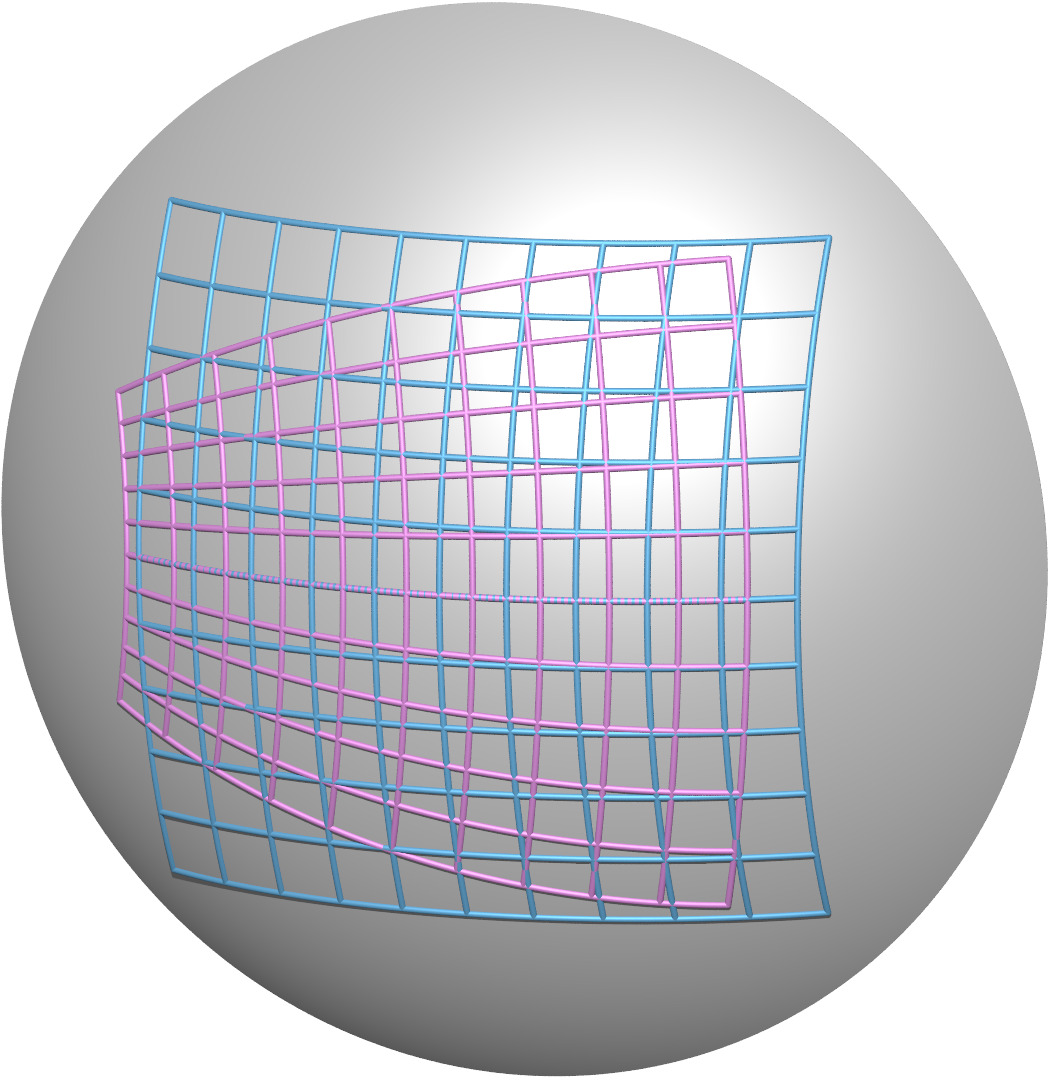
\includegraphics[width=7.0cm]{parallel.jpg}};

% Gitter
\ifthenelse{\boolean{showgrid}}{
\draw[step=0.1,line width=0.1pt] (-\breite,-\hoehe) grid (\breite, \hoehe);
\draw[step=0.5,line width=0.4pt] (-\breite,-\hoehe) grid (\breite, \hoehe);
\draw                            (-\breite,-\hoehe) grid (\breite, \hoehe);
\fill (0,0) circle[radius=0.05];
}{}


\node at (0,3) {$M$};
\node[color=darkred] at (-3.0,1.0) {$U_\alpha$};
\node[color=blue] at (2.3,2.1) {$U_\beta$};

\begin{scope}[yshift=-7cm]

\begin{scope}[xshift=-5.7cm]
	\draw[<-,color=darkred] (2.5,2.7) to[out=90,in=-110] ++(0.45,4.2);
	\node[color=darkred] at ($(2.5,2.7)+(0,1.4)$) [left] {$\varphi_\alpha$};
	\draw[->] (0,-2.6) -- (0,2.8) coordinate[label={right:$y^2$}];
	\draw[->] (-0.1,0) -- (5.4,0) coordinate[label={$y^1$}];
	\foreach \r in {0,0.5,...,5}{
		\draw[color=darkred] (\r,-2.5) -- (\r,2.5);
	}
	\foreach \y in {-2.5,-2,...,2.5}{
		\draw[color=darkred] (0,\y) -- (5,\y);
	}
	\node[color=darkred] at (4.75,2.25) {$V_\alpha$};
\end{scope}

\begin{scope}[xshift=3.2cm]
	\draw[<-,color=blue] (0,3.0) to[out=90,in=-40] ++(-1.3,3.6);
	\node[color=blue] at ($(0,2.7)+(0,1.4)$) [right] {$\varphi_\beta$};
	\draw[->] (-2.6,0) -- (2.8,0) coordinate[label={$x^1$}];
	\draw[->] (0,-2.6) -- (0,2.9) coordinate[label={right:$x^2$}];
	\foreach \x in {-2.5,-2,...,2.5}{
		\draw[color=blue] ({\x},-2.5) -- ({\x},2.5);
		\draw[color=blue] (-2.5,{\x}) -- (2.5,{\x});
	}
	\node[color=blue] at (2.25,2.25) {$V_\beta$};
\end{scope}

\end{scope}

\end{tikzpicture}

\end{document}

